
\documentclass[11pt,a4paper]{article}
\usepackage[utf8]{inputenc}
\usepackage[T1]{fontenc}
\usepackage{graphicx}
\usepackage{booktabs}
\usepackage{geometry}
\usepackage{hyperref}
\usepackage{listings}
\usepackage{xcolor}
\usepackage{float}
\usepackage{parskip}
\usepackage{amsmath}

\geometry{margin=1in}

\definecolor{codegray}{rgb}{0.5,0.5,0.5}
\definecolor{codepurple}{rgb}{0.58,0,0.82}
\definecolor{backcolour}{rgb}{0.95,0.95,0.92}

\lstdefinestyle{mystyle}{
    backgroundcolor=\color{backcolour},   
    commentstyle=\color{codegray},
    keywordstyle=\color{magenta},
    numberstyle=\tiny\color{codegray},
    stringstyle=\color{codepurple},
    basicstyle=\ttfamily\footnotesize,
    breakatwhitespace=false,         
    breaklines=true,                 
    captionpos=b,                    
    keepspaces=true,                 
    numbers=left,                    
    numbersep=5pt,                  
    showspaces=false,                
    showstringspaces=false,
    showtabs=false,                  
    tabsize=2
}

\lstset{style=mystyle}

\title{\textbf{Technical Report: Fast-Growing Firms Prediction}}
\author{Data Analysis 3 - Assignment 2 \\ Submitted by: Balint Decsi (ID: 2506626), Zariza Chowdhury (ID: 2500086)}
\date{February 2026}

\begin{document}

\maketitle

\section{Introduction}
This technical report details the methodology, modeling choices, and evaluation results for predicting fast-growing firms using the Bisnode panel data (2010-2015). The code and full notebooks are available in the associated GitHub repository: \url{https://github.com/zarizachow/Data-Analysis-3}.

\section{Data Preparation \& Feature Engineering}

\subsection{Sample Design}
We utilized the \texttt{bisnode-firms} dataset. The cleaning process involved:
\begin{itemize}
    \item \textbf{Panel Construction:} We constructed a panel for 2010-2015.
    \item \textbf{Target Window:} The prediction target is defined over the 2012-2013 period.
    \item \textbf{Filtering:} We filtered for firms that were "alive" (positive sales) and had sales between 1,000 and 10 million EUR in the baseline year (2012).
\end{itemize}

\subsection{Target Variable}
The target \texttt{fast\_growth} is a binary variable representing the top decile of sales growth.
\[ \text{Growth} = \ln(\text{Sales}_{2013}) - \ln(\text{Sales}_{2012}) \]
Firms with growth $\ge 90^{th}$ percentile were labeled as \texttt{1}, others \texttt{0}. The base rate of the positive class is approx. 10\%.

\subsection{Features}
We engineered a rich set of features based on financial reports and firm characteristics:
\begin{itemize}
    \item \textbf{Financials:} Log sales, assets, liabilities, profit/loss ratios.
    \item \textbf{Growth:} Lagged sales growth (\texttt{d1\_sales\_mil\_log}).
    \item \textbf{Demographics:} Firm age, CEO age, region, industry category (\texttt{ind2\_cat}).
    \item \textbf{Quality Flags:} Flags for data errors or extreme values in accounting fields.
\end{itemize}
Missing numeric values were imputed with the mean, and categorical values with the mode. One-hot encoding was applied to categorical variables.

The relationship between firm size and growth is notably non-linear, as seen below. This supports the use of tree-based models like Random Forest.

\begin{figure}[H]
    \centering
    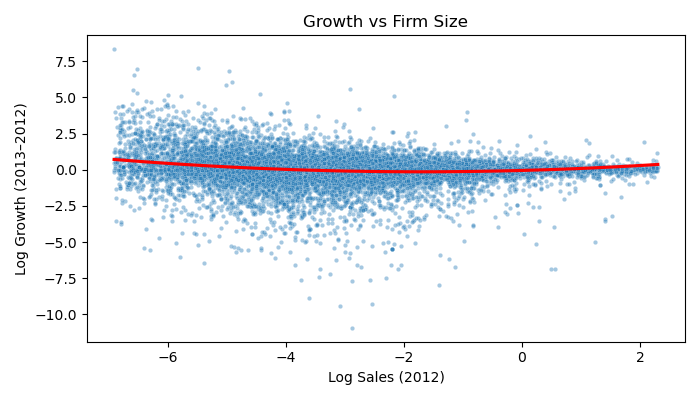
\includegraphics[width=0.7\textwidth]{Assignment-2/Output/Plots/growth_vs_size_2012.png}
    \caption{Growth vs. Firm Size (Log Sales)}
\end{figure}

\section{Modeling Strategy}

\subsection{Models}
We trained three models to predict the probability of fast growth:
\begin{enumerate}
    \item \textbf{Logistic Regression (L2):} Standard parametric baseline.
    \item \textbf{Logistic Regression (LASSO/L1):} For feature selection in high dimensions.
    \item \textbf{Random Forest:} Non-parametric ensemble to capture non-linearities (e.g., Age vs. Growth).
\end{enumerate}

\subsection{Evaluation}
We used 5-fold Stratified Cross-Validation.
\begin{itemize}
    \item \textbf{Part I (Probability):} Metrics included ROC-AUC, Average Precision, and Brier Score.
    \item \textbf{Part II (Classification):} We defined a loss function with $Cost(FN) = 4 \times Cost(FP)$.
\end{itemize}

\section{Results}

\subsection{Part I: Probability Prediction}
The Random Forest model significantly outperformed the linear models.

\begin{table}[H]
    \centering
    \begin{tabular}{lcccc}
        \toprule
        \textbf{Model} & \textbf{ROC-AUC} & \textbf{Avg Precision} & \textbf{Log Loss} & \textbf{Runtime (s)} \\
        \midrule
        \textbf{Random Forest} & \textbf{0.828} & \textbf{0.460} & \textbf{0.275} & $\sim 3.5$ \\
        Logit (LASSO) & 0.753 & 0.269 & 0.433 & $\sim 742$ \\
        Logit (L2) & 0.753 & 0.269 & 0.433 & $\sim 50$ \\
        \bottomrule
    \end{tabular}
    \caption{Cross-validated performance metrics.}
\end{table}

The Random Forest's superior performance (AUC 0.83 vs 0.75) highlights the importance of non-linear interactions in predicting firm growth.

\subsection{Part II: Classification \& Loss Minimization}
We optimized the classification threshold $t$ to minimize the expected loss:
\[ \text{Expected Loss} = \frac{1}{N} \sum (FP \times 1 + FN \times 4) \]

\begin{itemize}
    \item \textbf{Random Forest:} Minimized Loss = \textbf{0.255} at Threshold $\approx$ \textbf{0.15}.
    \item \textbf{Logit (L2):} Minimized Loss = 0.316 at Threshold $\approx$ 0.45.
\end{itemize}

The lower threshold for Random Forest reflects the high cost of false negatives; the model is calibrated to cast a wider net to catch the valuable fast-growers.

\subsection{Part III: Confusion Matrix}
Below is the confusion matrix for the Random Forest model (Fold 0) at the optimal threshold.

\begin{figure}[H]
    \centering
    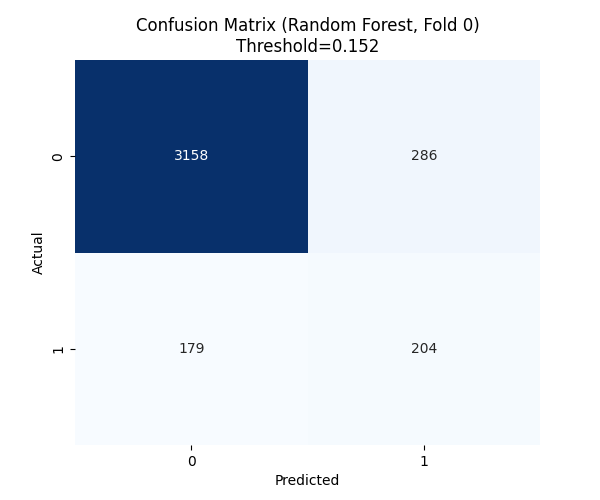
\includegraphics[width=0.6\textwidth]{Assignment-2/Output/Plots/confusion_matrix_rf.png}
    \caption{Confusion Matrix (Random Forest)}
\end{figure}

\subsection{Part IV: Industry Analysis}
We repeated the classification exercise for two subgroups:
\begin{enumerate}
    \item \textbf{Manufacturing:} AUC = 0.817, Expected Loss = 0.239
    \item \textbf{Services:} AUC = 0.838, Expected Loss = 0.257
\end{enumerate}
The model maintains high performance across both sectors, validating its generalizability.

\section{Code Snippet: Model Training}
\begin{lstlisting}[language=Python]
# Example pipeline construction
preprocess = ColumnTransformer(
    transformers=[
        ("num", numeric_transformer, num_cols),
        ("cat", categorical_transformer, cat_cols),
    ]
)

rf_model = RandomForestClassifier(
    n_estimators=300, 
    min_samples_leaf=10, 
    random_state=42, 
    n_jobs=-1
)

rf_pipe = Pipeline(steps=[("prep", preprocess), ("model", rf_model)])

# Cross-validation loop for loss minimization
for train_idx, test_idx in cv.split(X, y):
    rf_pipe.fit(X.iloc[train_idx], y.iloc[train_idx])
    probs = rf_pipe.predict_proba(X.iloc[test_idx])[:, 1]
    # ... threshold calculation ...
\end{lstlisting}

\section{Conclusion}
The Random Forest model is the clear choice for this prediction task. Its ability to model complex, non-linear relationships results in superior ranking capability (high AUC) and lower business risk (low Expected Loss).

\end{document}
